\documentclass[conference]{IEEEtran}
\usepackage{cite}
\usepackage{amsmath,amssymb,amsfonts}
\usepackage{graphicx}
\usepackage{booktabs}
\usepackage{array}
\usepackage{tabularx}
\usepackage{algorithm}
\usepackage{algpseudocode}
\usepackage{xcolor}
\usepackage{url}
\usepackage{tikz}
\usetikzlibrary{positioning,shapes.geometric,arrows.meta,fit,calc}
\graphicspath{{figures/}}

% ---------------------------------------------------------------------------
% Helper macros
% \cnum{1}  : circled module number used in Fig. 1 and in the text
%             (pdfLaTeX cannot typeset the Unicode character U+2460).
% \todo{..} : visible red marker for content the authors must still verify.
% \tbd      : short red marker for table cells awaiting verified numbers.
% Y         : ragged-right X column for the article summary table.
% ---------------------------------------------------------------------------
\DeclareRobustCommand{\cnum}[1]{\tikz[baseline=(c.base)]{\node[circle,draw,inner sep=0.6pt,minimum size=1.15em,font=\scriptsize\bfseries](c){#1};}}
\newcommand{\todo}[1]{\textcolor{red}{\textbf{[TODO: #1]}}}
\newcommand{\tbd}{\textcolor{red}{\textbf{TBD}}}
\newcolumntype{Y}{>{\raggedright\arraybackslash}X}

\begin{document}

\title{FMPA: A Store-Price-Anchored Domain AI Agent\\
for 7- and 14-Day Vegetable Price Forecasting}

% If ICEIB 2027 uses double-blind review, keep this block anonymous.
\author{\IEEEauthorblockN{Ya-Ting Yu}
\IEEEauthorblockA{Department of Computer Science and Engineering\\
National Chung Hsing University\\
Taichung, Taiwan\\
Email: jua91352@gmail.com}}

\maketitle

\begin{abstract}
% A = Attention getter (motivation)
After major typhoons and heavy rain in Taiwan, average wholesale vegetable
prices have risen by about 10--40\% in the first week and by up to about
100\% in the third week, yet shoppers seeing today's shelf price cannot tell
whether it will rise or fall.
% B = But (challenge)
Market averages are not store prices, retail prices are sticky but jump
abruptly, and large language models (LLMs) asked about prices may produce
unsupported numbers.
% C = Cure (proposed solution)
We propose the Fresh Market Price Forecast Agent (FMPA), a domain AI agent
that anchors short-term forecasts on the store price the user observes.
% D = Development (method)
FMPA restricts the LLM to intent parsing and explanation, obtains every number
through Model Context Protocol (MCP) tools, and estimates the relative price
change at 7 and 14 calendar days with RandomForest and HistGradientBoosting
models, applied to the store price (mode A) and, when a comparable same-store
price from the previous week exists, adjusted by a fixed rule (mode B).
% E = Experiments (evaluation)
We evaluate the forecasting core on one year of daily prices of three
vegetables in 13 public markets in Taichung City with a leakage-safe
chronological split (2,085 seven-day and 1,859 fourteen-day test samples),
against no-change and momentum baselines, using direction macro-F1 and the
mean absolute error of the relative change.
% F = Findings
The models reached macro-F1 of 0.422 and 0.417 but did not outperform the
momentum baseline, and their error exceeded that of the no-change baseline,
consistent with sticky retail prices. Future work will add event indicators
and uncertainty estimates and validate forecasts against matured same-store
prices.
\end{abstract}

\begin{IEEEkeywords}
LLM agent, Model Context Protocol, vegetable price forecasting, sticky prices,
forecasting baselines, decision support
\end{IEEEkeywords}

\section{Introduction}\label{sec:intro}

% G = General (current situation, with public evidence)
Fresh vegetables are among the most volatile items in Taiwanese household
spending. Typhoons and heavy rain regularly damage field crops and disrupt
shipments. An analysis by Taiwan's agricultural authority of six major
disasters in 2004--2009 found that average wholesale vegetable prices rose by
about 10--40\% in the first week after a disaster, 30--90\% in the second
week, and up to about 100\% in the third week~\cite{coa2010typhoon}. The
pattern persists: after Typhoon Gaemi in 2024, the average wholesale vegetable price
in Taipei reached NT\$57.5/kg, a five-year high~\cite{taiwannews2024gaemi}, and
in December 2024 vegetable prices in the consumer price index were 30.69\%
higher than a year earlier~\cite{ltn2025cpi}. During Typhoon Podul in August
2025, the wholesale price of green onions rose by about one third, and a stall
in a Taipei traditional market sold a single bundle for
NT\$380~\cite{ltn2025onion,pts2025onion}; that month, vegetables were 10.9\%
more expensive than a year before~\cite{taipeitimes2025cpi}. Price information
itself is plentiful: the Ministry of Agriculture publishes daily wholesale
quotations~\cite{moa2026trans}, and Taichung City publishes daily prices from
its 13 public retail markets~\cite{taichung2026retail}. Yet a shopper in front
of a stall sees only one number---today's price in this store---and must decide
whether to buy now or wait.

% H = However (challenges)
However, three properties of the problem make this decision hard to support
with data. First, public averages are not store prices: price changes pass from
wholesale to retail incompletely and
asymmetrically~\cite{ward1982asymmetry,meyer2004asymmetric}. Second, retail
prices are sticky: most prices stay unchanged for weeks or months and then
jump~\cite{bils2004some,nakamura2008five}. In our data, 86.7--92.8\% of
seven-day price pairs have exactly the same price at both ends, so a forecaster
that always predicts ``no change'' is hard to beat. Third, large language
models (LLMs) are attractive as a natural-language front end, but they can
generate fluent yet unsupported content~\cite{huang2025survey}, which is
unacceptable when the output is a price.

% I = In literature (categories of solutions, old to new)
In the literature, agricultural price forecasting has moved from statistical
models and early forecasting services built on open market
data~\cite{peng2015developing}, to tree
ensembles~\cite{breiman2001random,ke2017lightgbm}, deep sequence
models~\cite{zhang2024short}, and, most recently, LLM-based
forecasters~\cite{zhao2025vegetable}. In parallel, LLM agents have learned to
call external tools~\cite{yao2023react,schick2023toolformer}, and the Model
Context Protocol (MCP) now standardizes how agents connect to tools and
data~\cite{anthropic2024mcp}.

% J = Judgement (strengths and weaknesses)
These lines of work have complementary weaknesses. Forecasting studies predict
wholesale or market averages and often compare learned models with each other,
although large competitions show that simple methods are hard to
beat~\cite{makridakis2020m4} and that added complexity, including LLM
components, does not always help~\cite{zeng2023transformers,tan2024language}.
Agent studies, conversely, focus on language tasks and rarely address numeric
forecasting, where a model that computes or guesses numbers itself undermines
trust.

% K = Keypoint (design spirit, RQs, contributions)
This paper proposes the Fresh Market Price Forecast Agent (FMPA). Its design
spirit is: \emph{anchor on what the user sees, compute only with tools, and
evaluate against the strongest simple baseline.} We study three research
questions:
\begin{itemize}
\item \textbf{RQ1:} How well can the relative price change be forecast at
fixed horizons of 7 and 14 calendar days, compared with no-change and momentum
baselines?
\item \textbf{RQ2:} Does a weekly-momentum adjustment (mode B) add value over
pure store-price anchoring (mode A)?
\item \textbf{RQ3:} Is a tool-based LLM agent a feasible, low-effort interface
for consumer price queries?
\end{itemize}
The main contributions of this work are as follows:
\begin{itemize}
\item \textbf{C1 (RQ3):} a domain AI agent architecture in which the LLM only
parses intent, selects MCP tools, and explains results, while every price is
retrieved or computed by deterministic tools, with explicit errors when data
are missing;
\item \textbf{C2 (RQ1, RQ2):} a store-price-anchored forecasting formulation
with two modes, evaluated at fixed 7- and 14-day calendar horizons under a
leakage-safe protocol against strong naive baselines;
\item \textbf{C3 (RQ1):} an empirical finding on 13 public markets in Taichung
City that RandomForest and HistGradientBoosting models do not beat these
baselines, with a domain explanation based on price stickiness.
\end{itemize}

% L = List the organization
The rest of this paper is organized as follows. Section~\ref{sec:related}
reviews AI methods and domain knowledge and identifies the research gap.
Section~\ref{sec:method} presents the proposed scheme.
Section~\ref{sec:experiments} describes the experimental evaluation, and
Section~\ref{sec:conclusion} concludes the paper.

\section{Related Work}\label{sec:related}
% Course rule: about 1/2 AI technology (II-A) + 1/2 domain know-how (II-B).

% M = Methods, AI side (old to new, simple to complex)
\subsection{AI Technology for Price Forecasting and Agents}
\textit{Agricultural price forecasting.} Peng et
al.~\cite{peng2015developing} built an early crop-price forecasting service on
open data from Taiwan's wholesale markets, comparing ARIMA, partial least
squares, and neural networks. Zhang et al.~\cite{zhang2024short} trained an
LSTM on daily prices of six vegetables from seven Beijing wholesale markets and
reported higher accuracy than several machine-learning baselines. Zhao et
al.~\cite{zhao2025vegetable} found that LLM-based forecasters generally
outperform traditional and deep models, but not consistently across vegetables
and time scales, and proposed a mixture of experts. All of these works forecast
wholesale or market averages.

\textit{Tree ensembles and simple baselines.} Random
forests~\cite{breiman2001random} and histogram-based gradient
boosting~\cite{ke2017lightgbm} are strong, data-efficient learners for tabular
features such as recent price changes. However, in the M4 competition, pure
machine-learning methods performed poorly compared with simple statistical
benchmarks~\cite{makridakis2020m4}; a one-layer linear model can beat
Transformer forecasters~\cite{zeng2023transformers}; and removing the LLM from
LLM-based forecasters often does not reduce accuracy~\cite{tan2024language}.
Reliable evaluation must also prevent future information from leaking into
training~\cite{kaufman2012leakage}.

\textit{LLM agents and tool use.} ReAct interleaves reasoning with tool actions
and reduces hallucination in knowledge-intensive tasks~\cite{yao2023react};
Toolformer teaches a model to call APIs such as a
calculator~\cite{schick2023toolformer}. Hallucination nevertheless remains an
open problem~\cite{huang2025survey}. MCP~\cite{anthropic2024mcp} offers an
open, standard way for an agent host to call tool servers, which FMPA uses to
keep all numeric work outside the LLM.

% M = Methods, domain side
\subsection{Domain Knowledge of Fresh Produce Prices}
\textit{Price stickiness.} Retail prices change infrequently: about half of US
consumer prices last less than 4.3 months~\cite{bils2004some}, regular prices
are even more rigid once temporary sales are excluded~\cite{nakamura2008five},
and grocery retailers keep sticky reference prices~\cite{eichenbaum2011reference}.
A no-change forecast is therefore a natural and strong baseline.

\textit{Price transmission.} For fresh vegetables, wholesale prices lead retail
prices and the pass-through is asymmetric~\cite{ward1982asymmetry}; asymmetric
transmission along food supply chains is common~\cite{meyer2004asymmetric}. A
public market average is thus an imperfect proxy for the price in a particular
store.

\textit{Weather shocks and volatility.} Food prices are volatile, and their
volatility must be measured carefully~\cite{gilbert2010food}. In Taiwan,
typhoon warnings raise demand through expectations and stockpiling while
landfall cuts supply, with effects that differ by crop~\cite{yu2022market}; in
the largest cabbage wholesale market, typhoons raise prices, and repeated
storms make the response start earlier and last longer~\cite{su2025food}.

\textit{Public price data.} Taiwan publishes daily wholesale prices and
volumes~\cite{moa2026trans}, and Taichung City publishes daily average prices
of fruits and vegetables in 13 public retail markets, in NT\$ per catty
(600\,g)~\cite{taichung2026retail}. Units differ across sources (per kilogram,
per catty, per bundle), which motivates explicit unit conversion and validation (M1 in
Section~\ref{sec:method}).

% N = New proposed (gap -> our project)
\subsection{Research Gap}
Table~\ref{tab:summary} summarizes representative works.
\textit{Existing research} forecasts wholesale or market averages with
increasingly complex models, studies LLM agents mainly on language tasks, and
explains price formation in economics. \textit{Limitations:} (i) no forecast is
anchored on the price the consumer actually observes; (ii) few studies evaluate
at fixed calendar horizons against no-change and momentum baselines under
leakage control; and (iii) LLM-based systems may let the language model
produce numbers. \textit{Research gap and our project:} FMPA addresses (i)
with store-price anchoring, Eq.~\eqref{eq:modeA}; (ii) with the evaluation
protocol of Section~\ref{sec:experiments}; and (iii) with an MCP tool boundary
that keeps every number outside the LLM (Fig.~\ref{fig:architecture}).

% O = Organize: Article Summary Table at the end of Section II.
% A two-column table* can only float to the top of the next page in IEEEtran.
% Table I -- 8-column article summary required by the course proposal rules.
% "Limitation" is written relative to the FMPA problem setting.
\begin{table*}[t]
\caption{Article summary of representative related work}
\label{tab:summary}
\centering
\scriptsize
\setlength{\tabcolsep}{3pt}
\renewcommand{\arraystretch}{1.12}
\begin{tabularx}{\textwidth}{@{}l c Y Y Y Y Y Y@{}}
\toprule
Ref. & Year & Problem & AI Method & Domain Knowledge & Dataset & Findings & Limitation \\
\midrule
\cite{peng2015developing} & 2015 & Crop price forecasting service & ARIMA, PLS, ANN & Wholesale market open data & Daily prices of four crops, Taiwan & PLS suits short, ANN long horizons & Wholesale only; no store anchor \\
\cite{zhang2024short} & 2024 & Short-term vegetable prices & LSTM vs.\ ML models & Wholesale vegetable markets & 6 vegetables, 7 Beijing markets, 2009--2023 & LSTM most accurate ($R^2=0.958$) & Market averages; compared with learned models \\
\cite{zhao2025vegetable} & 2025 & Vegetable price forecasting & Mixture of LLM and deep experts & Vegetables differ in price dynamics & Vegetable price series & LLMs often best, but inconsistent & No store prices; no agent interface \\
\cite{makridakis2020m4} & 2020 & Which forecasting methods work & 61 statistical, ML, hybrid methods & Naive benchmarks as reference & 100,000 series & Pure ML weak vs.\ simple benchmarks & Not food or retail prices \\
\cite{tan2024language} & 2024 & Are LLMs useful for forecasting & Ablation of LLM components & -- & Standard benchmarks & Removing the LLM does not hurt & Not price data \\
\cite{yao2023react} & 2023 & Ungrounded LLM reasoning & Reasoning + tool actions & -- & QA, fact checking, interactive tasks & Tool calls reduce hallucination & No numeric forecasting \\
\cite{nakamura2008five} & 2008 & How often prices change & -- (descriptive statistics) & Sales vs.\ regular prices & US CPI/PPI microdata & Regular prices are rigid & US data; not produce-specific \\
\cite{ward1982asymmetry} & 1982 & Vegetable price linkages & -- (asymmetry tests) & Wholesale leads retail & US fresh vegetables & Asymmetric pass-through & Old; US markets \\
\cite{meyer2004asymmetric} & 2004 & Asymmetric price transmission & -- (survey of econometric tests) & Farm--wholesale--retail chain & Literature & Asymmetry is common & No forecasting \\
\cite{yu2022market} & 2022 & Typhoon effects on prices & -- (econometric decomposition) & Warning raises demand, landfall cuts supply & Taiwan wholesale vegetables, 1996--2014 & Prices rise; effects vary by crop & Wholesale; pre-2015 data \\
\cite{su2025food} & 2025 & Disaster shocks on food markets & -- (event study, DiD) & Expectations, stockpiling, imports & Daily cabbage, Taiwan's largest wholesale market & Repeated typhoons: earlier, longer response & Cabbage only \\
\midrule
FMPA & 2026 & Store-anchored 7/14-day forecast & LLM + MCP tools; RF/HGB & Stickiness, label maturity, unit normalization & 13 Taichung public markets & Models do not beat naive baselines & Public price $\neq$ store price \\
\bottomrule
\end{tabularx}
\end{table*}


\section{Proposed Scheme}\label{sec:method}

% PA = Aim
\subsection{Design Aim}
Given a natural-language query that names a vegetable $v$, a store or market
$s$, and the price $P_t$ the user observes on day $t$, FMPA returns, for a
horizon $h\in\{7,14\}$ calendar days, a forecast price $\hat{P}_{t+h}$, the
predicted direction of change (down, flat, or up), and a short explanation of
the evidence. When the evidence is insufficient, FMPA returns a clarification
request or an explicit error instead of a number.

% PB = Based on (domain mindsets), PC = Cure (why the design helps)
\subsection{Design Principles from Domain Knowledge}
The design is based on five domain mindsets (M1--M5) that we distilled from
the literature in Section~\ref{sec:related} and from our data; each maps to a
system component.
\begin{itemize}
\item \textbf{M1 Price comparability first.} Prices are only comparable after
units and specifications (e.g., per bundle vs.\ per catty) are normalized
$\rightarrow$ a \texttt{normalize\_spec} tool.
\item \textbf{M2 Temporal integrity.} A target at $t+h$ may be used for
training only after it has matured; in our data, 1{,}386 immature samples were
conservatively removed $\rightarrow$ a label-maturity filter in the training
pipeline.
\item \textbf{M3 Simple baselines first.} Because most retail prices do not
change within a week~\cite{nakamura2008five}, every forecast is reported next
to no-change and momentum baselines $\rightarrow$ baselines are computed by the
ForecastEngine.
\item \textbf{M4 Public $\neq$ private.} Public market averages describe a
trend, not the price in a given store~\cite{meyer2004asymmetric}
$\rightarrow$ store-price anchoring \eqref{eq:modeA}.
\item \textbf{M5 Error $\neq$ utility.} A small average error does not imply a
better purchase decision $\rightarrow$ the output shows direction and evidence,
not only a point value.
\end{itemize}

% PD = Design, PE = Paper elements, PG = Graph
\subsection{System Architecture}
Fig.~\ref{fig:architecture} shows the five modules of FMPA.

\cnum{1}~\textit{User entry.} A web prototype and chat interface receive the
query. An LLM extracts the intent $(v, s, P_t, h, \text{mode})$, selects tools,
and finally explains the returned results in plain language. It is the only
module that uses the LLM.

\cnum{2}~\textit{MCP tools.} Typed tools exposed through the Model Context
Protocol~\cite{anthropic2024mcp}---\texttt{get\_history},
\texttt{normalize\_spec}, and \texttt{forecast}---validate their arguments and
return JSON. The LLM can obtain a number only through these tools.

\cnum{3}~\textit{Oracle host API.} A REST service on a cloud host serves the
tools, keeping data access and model inference outside the LLM context.

\cnum{4}~\textit{ForecastEngine.} A RandomForest~\cite{breiman2001random}
model for $h=7$ and a HistGradientBoosting model~\cite{ke2017lightgbm} for
$h=14$, both implemented with scikit-learn~\cite{pedregosa2011scikit},
estimate the relative change; the engine then applies mode A or B and computes
the baselines.

\cnum{5}~\textit{Public historical data.} Daily price records from 13 public
markets in Taichung City are used for features, training, and evaluation.

\begin{figure}[t]
\centering
% Fig. 1 -- FMPA system architecture (modules 1-5). Single-column TikZ figure.
% Module numbers must match the description in sections/03_proposed_scheme.tex.
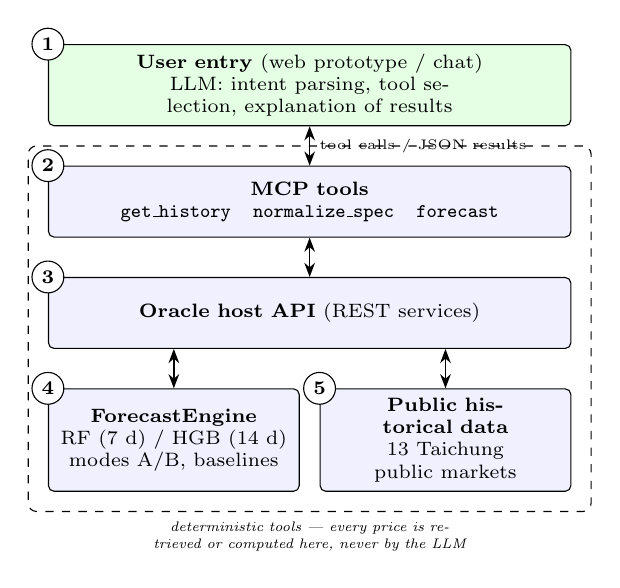
\begin{tikzpicture}[
  font=\scriptsize,
  mod/.style={draw, rounded corners=2pt, align=center, text width=#1,
              minimum height=9mm, fill=blue!6},
  mod/.default=6.4cm,
  llm/.style={mod=#1, fill=green!10},
  llm/.default=6.4cm,
  num/.style={circle, draw, fill=white, inner sep=0.6pt, minimum size=1.15em,
              font=\scriptsize\bfseries},
  biarr/.style={{Stealth[length=1.8mm]}-{Stealth[length=1.8mm]}, semithick}
]
\node[llm] (entry) {\textbf{User entry} (web prototype / chat)\\
  LLM: intent parsing, tool selection, explanation of results};
\node[mod, below=5mm of entry] (mcp) {\textbf{MCP tools}\\
  \texttt{get\_history}\quad\texttt{normalize\_spec}\quad\texttt{forecast}};
\node[mod, below=5mm of mcp] (api) {\textbf{Oracle host API} (REST services)};
\node[mod=2.95cm, minimum height=13mm, anchor=north west] (engine)
  at ([yshift=-5mm]api.south west) {\textbf{ForecastEngine}\\
  RF (7 d) / HGB (14 d)\\ modes A/B, baselines};
\node[mod=2.95cm, minimum height=13mm, anchor=north east] (data)
  at ([yshift=-5mm]api.south east) {\textbf{Public historical data}\\
  13 Taichung public markets};

\node[num] at (entry.north west) {1};
\node[num] at (mcp.north west) {2};
\node[num] at (api.north west) {3};
\node[num] at (engine.north west) {4};
\node[num] at (data.north west) {5};

\draw[biarr] (entry) -- node[right, font=\tiny]{tool calls / JSON results} (mcp);
\draw[biarr] (mcp) -- (api);
\draw[biarr] (api.south -| engine.north) -- (engine.north);
\draw[biarr] (api.south -| data.north) -- (data.north);

\node[draw, dashed, rounded corners=3pt, inner sep=2.5mm,
      fit=(mcp)(api)(engine)(data),
      label={[font=\tiny\itshape, anchor=north, align=center, text width=6.4cm]%
      south:{deterministic tools --- every price is retrieved or computed here,
      never by the LLM}}] {};
\end{tikzpicture}

\caption{FMPA architecture. The LLM (green) only parses intent and explains
results; modules \cnum{2}--\cnum{5} inside the dashed box retrieve or compute
every number.}
\label{fig:architecture}
\end{figure}

% PF = Formulation
\subsection{Problem Formulation}
Table~\ref{tab:notation} lists the notation. Let $M_t$ be the public market
price of $v$ on day $t$. The learning target is the relative change of the
market price over $h$ calendar days,
\begin{equation}
\Delta_{t,h}=\frac{M_{t+h}-M_t}{M_t},
\label{eq:delta}
\end{equation}
and the ForecastEngine outputs an estimate $\hat{\Delta}_{t,h}$.

\textit{Mode A (store-price anchoring)} transfers the estimated relative change
to the price the user actually sees:
\begin{equation}
\hat{P}^{(A)}_{t+h}=P_t\,\bigl(1+\hat{\Delta}_{t,h}\bigr).
\label{eq:modeA}
\end{equation}

\textit{Mode B (weekly momentum adjustment)} adds a fixed fraction of the most
recent weekly momentum $m_t=(M_t-M_{t-7})/M_{t-7}$:
% VERIFY(author): confirm this exact form of mode B against the DIC3
% ForecastEngine code before submission.
\begin{equation}
\hat{P}^{(B)}_{t+h}=P_t\,\bigl(1+\hat{\Delta}_{t,h}+\alpha\, m_t\bigr),
\qquad \alpha=0.3 .
\label{eq:modeB}
\end{equation}
The coefficient $\alpha$ is fixed in advance and is not tuned on test data.

\begin{table}[t]
\caption{Notation}
\label{tab:notation}
\centering
\footnotesize
\begin{tabular}{@{}ll@{}}
\toprule
Symbol & Meaning \\
\midrule
$t$, $h$ & query day; horizon $h\in\{7,14\}$ calendar days \\
$P_t$ & price observed by the user in store $s$ on day $t$ \\
$M_t$ & public market price of vegetable $v$ on day $t$ \\
$\Delta_{t,h}$, $\hat{\Delta}_{t,h}$ & true and estimated relative change, Eq.~\eqref{eq:delta} \\
$m_t$ & weekly momentum $(M_t-M_{t-7})/M_{t-7}$ \\
$\alpha$ & fixed momentum weight in mode B ($0.3$) \\
$\theta$ & intent-confidence threshold of the agent \\
$\hat{P}^{(A)}_{t+h}$, $\hat{P}^{(B)}_{t+h}$ & forecasts of modes A and B \\
\bottomrule
\end{tabular}
\end{table}


% PJ = Jump to an example
\textit{Example.} A user reports green onions at NT\$380 per bundle, the
price reported in Taipei during Typhoon Podul~\cite{pts2025onion}. If the
engine returns $\hat{\Delta}_{t,7}=+2.4\%$, mode A gives
$\hat{P}^{(A)}_{t+7}=380\times1.024\approx$ NT\$389. The numbers in this
example are illustrative and are not experimental results.

% PH = How, PI = Implementation (flowchart + pseudocode)
\subsection{Processing Flow and Algorithm}
Fig.~\ref{fig:flowchart} shows the processing flow from input to output. The
check after intent parsing is the key safety step: if no matching history is
found, or the intent confidence is below $\theta$, FMPA asks the user for
clarification or reports ``no data'' rather than letting the LLM guess.
Algorithm~\ref{alg:fmpa} gives the corresponding pseudocode. Lines 2 and 13
are the only LLM calls; the forecast value is produced by tools in lines
11--12.

\begin{figure}[t]
\centering
% Fig. 2 -- FMPA processing flow: Input -> Check -> AI/Analytics -> Decision -> Output.
% The "no" branch of the check asks for missing fields or returns an explicit error.
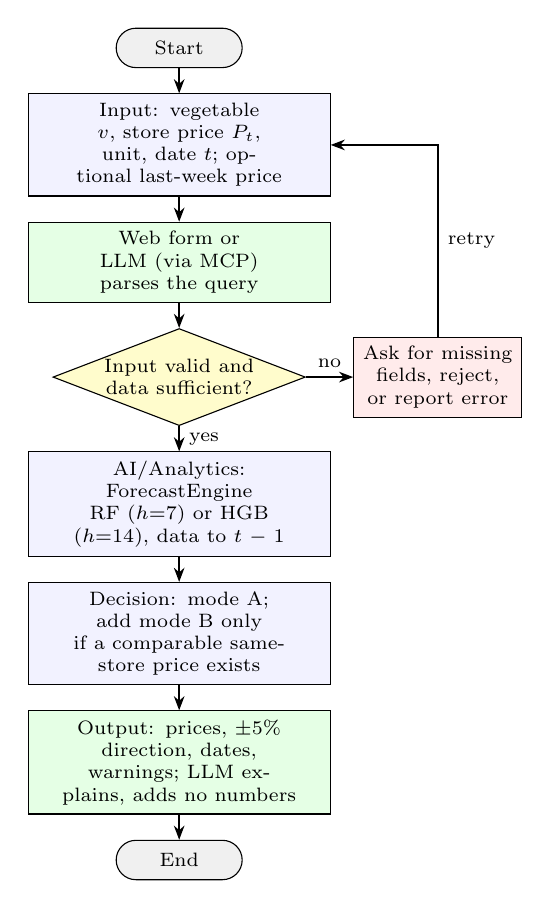
\begin{tikzpicture}[
  font=\scriptsize,
  node distance=3.2mm,
  proc/.style={draw, rectangle, align=center, text width=3.6cm,
               minimum height=6mm, fill=blue!5},
  llm/.style={proc, fill=green!10},
  term/.style={draw, rounded corners=2.5mm, minimum width=1.6cm,
               minimum height=5mm, fill=gray!12},
  dec/.style={draw, diamond, aspect=2.6, align=center, inner sep=0.5pt,
              fill=yellow!20},
  err/.style={draw, rectangle, align=center, text width=1.9cm,
              minimum height=6mm, fill=red!8},
  arr/.style={-{Stealth[length=1.8mm]}, semithick}
]
\node[term] (start) {Start};
\node[proc, below=of start] (in) {Input: vegetable $v$, store price $P_t$,\\
  unit, date $t$; optional last-week price};
\node[llm, below=of in] (parse) {Web form or LLM (via MCP)\\ parses the query};
\node[dec, below=of parse] (chk) {Input valid and\\ data sufficient?};
\node[proc, below=of chk] (ai) {AI/Analytics: ForecastEngine\\
  RF ($h{=}7$) or HGB ($h{=}14$), data to $t-1$};
\node[proc, below=of ai] (decide) {Decision: mode A; add mode B only\\
  if a comparable same-store price exists};
\node[llm, below=of decide] (out) {Output: prices, $\pm5\%$ direction, dates,\\
  warnings; LLM explains, adds no numbers};
\node[term, below=of out] (end) {End};
\node[err, right=6mm of chk] (err) {Ask for missing fields, reject, or report
  error};

\draw[arr] (start) -- (in);
\draw[arr] (in) -- (parse);
\draw[arr] (parse) -- (chk);
\draw[arr] (chk) -- node[right]{yes} (ai);
\draw[arr] (ai) -- (decide);
\draw[arr] (decide) -- (out);
\draw[arr] (out) -- (end);
\draw[arr] (chk) -- node[above]{no} (err);
\draw[arr] (err.north) |- node[pos=0.25, right]{retry} (in.east);
\end{tikzpicture}

\caption{Processing flow of FMPA: Input $\rightarrow$ Check $\rightarrow$
AI/Analytics $\rightarrow$ Decision $\rightarrow$ Output, with a
clarification/error branch.}
\label{fig:flowchart}
\end{figure}

\begin{algorithm}[t]
\caption{FMPA query handling}
\label{alg:fmpa}
\begin{algorithmic}[1]
\Require user query $q$ (text), threshold $\theta$, mode $\in\{A,B\}$
\Ensure response $R$ (forecast, direction, explanation) or an error
\State $u \gets \Call{Preprocess}{q}$
\State $(v, s, P_t, h) \gets \Call{LLM.ParseIntent}{u}$
\While{$\Call{Confidence}{v, s, P_t, h} < \theta$}
  \State ask the user for clarification; update $(v, s, P_t, h)$
\EndWhile
\State $D \gets \Call{Tool.GetHistory}{v, s, t}$ \Comment{MCP tool}
\If{$D = \emptyset$}
  \State \Return error ``no matching data''
\EndIf
\State $P_t \gets \Call{Tool.NormalizeSpec}{P_t, v}$
\State $\hat{\Delta}_{t,h} \gets \Call{Tool.Forecast}{D, h}$ \Comment{RF or HGB}
\State $\hat{P}_{t+h} \gets$ Eq.~\eqref{eq:modeA} or \eqref{eq:modeB}; compute baselines
\State $R \gets \Call{LLM.Explain}{\hat{P}_{t+h}, \hat{\Delta}_{t,h}, \text{baselines}}$
\State \Return $R$
\end{algorithmic}
\end{algorithm}

% PK = Key points, PL = Later how to simulate
\subsection{Key Points}
FMPA differs from a price chatbot in three ways: (i) the forecast is anchored
on the store price the user observes rather than on a market average;
(ii) horizons are fixed calendar days, so every forecast can later be checked
against the real price on day $t+h$; and (iii) the LLM never produces a price.
Section~\ref{sec:experiments} evaluates the forecasting core against strong
simple baselines.

\section{Experimental Evaluation}\label{sec:experiments}

% S = Simulation setup
\subsection{Dataset and Setup}
We use the daily average prices of three vegetables---cabbage, bok choy, and
sponge gourd---in the 13 public retail markets of Taichung
City~\cite{taichung2026retail}, from 2025-10-04 to 2026-10-02, in NT\$ per
catty (600\,g). The publisher uses a price of zero to mean that no price was
recorded; such entries are treated as missing, never as a $-100\%$ change.
Each sample is a (market, vegetable, day $t$) triple whose target is the
relative change $r_h$ of \eqref{eq:delta}, paired on the exact date $t+h$.

The split is chronological and grouped by date, so all markets of one day fall
in the same part: training from 2025-10-04 to 2026-05-08, validation from
2026-05-10 to 2026-07-21, and a held-out test period from 2026-07-22 to
2026-10-02 (73 dates). Assuming a one-day publication delay, a label matures at
$t+h+1$; 1{,}386 rows whose labels crossed a split boundary (695 and 691 at the
two boundaries) were purged to prevent leakage~\cite{kaufman2012leakage}. After
requiring complete features and matured labels, the test sets contain
$n=2{,}085$ samples for $h=7$ and $n=1{,}859$ samples for $h=14$.

Each sample has 12 numeric features built only from data published by
$t-1$---the last visible price and its age, 7-, 14-, and 28-day moving
averages, 14-day volatility and range, 7- and 14-day momentum, weekday, and
month---plus a one-hot encoding of the vegetable; the market identity is not
used. Models are implemented in Python~3.12 with
scikit-learn~1.9.1~\cite{pedregosa2011scikit}.

% Q = Quality and quantity (metrics), R = Related methods to compare
\subsection{Baselines and Metrics}
Three simple baselines are used, following the forecasting practice of always
comparing with naive methods~\cite{makridakis2020m4}:
\begin{itemize}
\item \textit{No-change (persistence):} $\hat{r}_h=0$, i.e., the price stays
as it is.
\item \textit{Momentum:} the latest visible change of the market price over
the past $h$ days continues (missing values treated as $0$).
\item \textit{Train mean by crop:} the mean training-set $r_h$ of each
vegetable and horizon.
\end{itemize}

\textit{Direction macro-F1.} Each change is mapped to a class
$c\in\mathcal{C}=\{\text{down},\text{flat},\text{up}\}$ with the flat band
$\tau=5\%$ of Section~\ref{sec:method}. The band was frozen before the test
period was examined: prices are integers in NT\$ per catty, typically 25--60,
so a one-dollar step is already 2--4\% and a change within $\pm5\%$ does not
alter a purchase decision. With $F_1^{(c)}$ the F1-score of class $c$,
\begin{equation}
\text{macro-F1}=\frac{1}{|\mathcal{C}|}\sum_{c\in\mathcal{C}}F_1^{(c)} .
\label{eq:f1}
\end{equation}
Macro averaging prevents the dominant ``flat'' class from hiding errors on the
rare but important up and down moves.

\textit{Relative-change MAE.}
\begin{equation}
\text{MAE}=\frac{1}{n}\sum_{i=1}^{n}\bigl|r_i-\hat{r}_i\bigr| .
\label{eq:mae}
\end{equation}
Higher macro-F1 and lower MAE are better; MAE is measured on the market's
relative change, not in NT\$ and not on store prices.

% T = Tuning parameters
\subsection{Parameter Settings}
Ridge, RandomForest, and HistGradientBoosting regressors and two direction
classifiers were trained, and the model with the best validation macro-F1 was
selected for each horizon: a RandomForest with 300 trees and at least 5 samples
per leaf for $h=7$, and a HistGradientBoosting regressor with 200 iterations and
learning rate 0.05 for $h=14$, both with random seed 42. Each model predicts
$\hat{r}_h$, which is then classified with $\tau$. The mode-B weight is fixed at
$\alpha=0.3$. The test period was used only once and played no part in tuning.

% U = Useful results
\subsection{Results}
Table~\ref{tab:comparison} compares the selected models with the baselines.
Both models carry some directional signal: their macro-F1 (0.422 at 7 days and
0.417 at 14 days) is well above that of the no-change baseline (0.309 and
0.295), which predicts ``flat'' for every sample. However, neither beats the
momentum baseline (0.423 and 0.431), and their relative-change MAE (0.066 and
0.098) is worse than that of the no-change baseline (0.044 and 0.075). Recall on
the rare up class is only 10.1\% (16 of 158) at 7 days and 8.6\% (23 of 268) at
14 days. We report these negative results as they are.

% TODO(author): copy the verified values from the DIC3 experiment logs and
% delete every \tbd. Do NOT reuse numbers from the AI-generated infographic:
% they contradict the written finding (see paper/README.md).
\begin{table}[t]
\caption{Results on the held-out test sets (values pending verification)}
\label{tab:comparison}
\centering
\footnotesize
\begin{tabular}{@{}llcc@{}}
\toprule
Horizon & Method & Macro-F1 $\uparrow$ & MAE $\downarrow$ \\
\midrule
7 days ($n=2{,}085$) & No-change & \tbd & \tbd \\
 & Momentum & \tbd & \tbd \\
 & RF, mode A & \tbd & \tbd \\
 & RF, mode B & \tbd & \tbd \\
\midrule
14 days ($n=1{,}859$) & No-change & \tbd & \tbd \\
 & Momentum & \tbd & \tbd \\
 & HGB, mode A & \tbd & \tbd \\
 & HGB, mode B & \tbd & \tbd \\
\bottomrule
\end{tabular}
\end{table}


% V = Verify effectiveness (discussion)
\subsection{Discussion}
\textit{Why are the baselines hard to beat?} In our data, 86.7--92.8\% of
seven-day price pairs have exactly the same price at both ends, depending on
the vegetable, and only 10.5\% of seven-day changes leave the $\pm5\%$ band.
Such sticky series~\cite{nakamura2008five,bils2004some} make ``no change''
close to optimal for absolute error, while momentum captures the few
persistent moves, for example after a typhoon. This agrees with large
forecasting studies in which simple methods remain
competitive~\cite{makridakis2020m4,zeng2023transformers}.

\textit{RQ1.} At both 7 and 14 days, the evidence does not support using the
learned forecasts alone; the momentum signal should be shown to the user next
to them.

\textit{RQ2.} Mode A preserves the predicted direction by construction
(Section~\ref{sec:method}), so it cannot improve the direction metrics on
public data. Whether mode B adds value cannot be tested here, because the
public data contain no store prices; this requires matured same-store prices
collected after each query, which has not yet started.

\textit{RQ3.} The web prototype and the MCP tools answer a query with dated
7- and 14-day results, and every number shown comes from a tool call. This
shows that low-effort querying is technically feasible; a user study is still
needed to measure usefulness.

\textit{Threats to validity.} The target is the public market price, which is
only a proxy for the price in a specific store; the data cover three
vegetables in one city over one year; and the direction metric depends on the
5\% band.

\section{Conclusion}\label{sec:conclusion}

% W = What proposed
This paper presented FMPA, a domain AI agent that helps consumers judge whether
a vegetable price they see today is likely to change in the next 7 or 14 days.
It addresses three challenges: public averages are not store prices, retail
prices are sticky with rare jumps, and LLMs should not invent numbers.

% X = eXcel (where it fits)
FMPA is designed for the moment of purchase: it anchors forecasts on the
observed store price, uses fixed calendar horizons that can later be checked,
and keeps every number inside deterministic MCP tools, with explicit errors
when data are missing.

% Y = Yields
For three vegetables in 13 public markets in Taichung City, RandomForest and
HistGradientBoosting models reached direction macro-F1 of 0.422 and 0.417,
above the no-change baseline but below momentum (0.423 and 0.431), and their
relative-change MAE was worse than that of the no-change baseline. The current
value of FMPA therefore lies in its transparent, store-anchored presentation of
forecasts and baselines, not in superior accuracy.

% Z = Zen (limitations and future work)
The main limitations are that public market prices are only a proxy for
individual store prices and that the benefit of mode B is still unproven.
Future work will collect matured same-store prices for paired validation of
modes A and B; add feature engineering and event
indicators, such as typhoon warnings and arrival volumes; attach uncertainty
estimates to every forecast; and run a user study of the agent interface.


\section*{Acknowledgment}
% A2Z / course rule: disclose AI assistance.
The authors used AI assistants (ChatGPT, Claude Code, and Google Antigravity
with an Overleaf MCP connection) for literature search, drafting, and \LaTeX{}
editing. All references, numbers, and claims were checked by the authors, who
take full responsibility for the content.

\bibliographystyle{IEEEtran}
\bibliography{references}

\end{document}
